\documentclass[conference]{IEEEtran}
\IEEEoverridecommandlockouts
% The preceding line is only needed to identify funding in the first footnote. If that is unneeded, please comment it out.
\usepackage{cite}
\usepackage{amsmath,amssymb,amsfonts}
\usepackage{algorithmic}
\usepackage{graphicx}
\usepackage{textcomp}
\usepackage{xcolor}
\usepackage{cleveref}
\usepackage{url}
\usepackage{subfig}
\def\BibTeX{{\rm B\kern-.05em{\sc i\kern-.025em b}\kern-.08em
    T\kern-.1667em\lower.7ex\hbox{E}\kern-.125emX}}
\begin{document}

\title{Ownership Protection in Machine Learning Processes}

\author{\IEEEauthorblockN{Tanja Šarčević}
\IEEEauthorblockA{\textit{SBA Research} and \textit{Vienna University of Technology} \\
Vienna, Austria \\
tsarcevic@sba-research.org \\ 
DOI: 0000-0003-0896-9193}
}

\maketitle

\begin{abstract}
Outsourcing and shifting data storage and complex Machine Learning models to cloud services witnessed great growth over the past years, as costs of producing, maintaining and processing data can be decreased this way. 
However, sharing
these assets entails potential intellectual property (IP) theft, and existing mechanisms for IP protection are susceptible to attacks. 
Our work develops methods for protecting IP privacy on multiple levels of the Machine Learning process, i.e. IP protection of shared input data and IP protection of derived Machine Learning models. 
The research results provide novel schemes for IP protection and better insights into the effects of these schemes on the quality and utility of the affected intellectual property assets.
\end{abstract}

\section{Introduction}
%general
Sharing digital assets is as old as digital data itself. 
Data creators are sharing data for commercial reasons, for increasing their reputation for valuable creations or information, for research reasons, to support the preservation of data long-term, etc. 
And over the last decades, the trend of sharing and processing digital data has vastly increased. 
Since data is a valuable asset to its owner, any type of unauthorised usage of shared data should be detected and sanctioned.
With the advances in the area of Machine Learning (ML), outsourcing data and processing thereof became an increasingly popular trend among businesses. 
In this scope, the data is given to data management professionals that are involved in data mining, data classification etc., to make more use of the data more. 
This can foster business growth by additional services (recommendation systems) or customer behaviour understanding. 
In healthcare, for example, medical data are shared with researchers for help in medical diagnosis or other types of services that ML may provide.
Furthermore, sharing the Machine Learning models has an increasing popularity through the online services such as Machine-Learning-as-a-Service (MLaaS). 
These platforms facilitate development, especially for researchers and small or medium businesses because in many ML settings, training an effective model from scratch requires a lot of computational power, human expertise and amount of data (e.g. natural language processing, image processing, etc.)  
In line with this, the model owners that have invested significant resources to train a model consider IP protection methods to verify the ownership or prevent unauthorised usage of a model. 

\textit{Digital watermarking} and \textit{fingerprinting} are approaches for protecting ownership of various types of digital property, including those relevant in ML process - data and ML models. 
By embedding a mark into a digital object these methods enable the owners to share these objects in their full form while enabling ownership claim and/or tracing recipients.
Watermarking enables the owner of an object to verify their ownership, while fingerprinting, in addition, allows tracing the source of the unauthorised usage, i.e. the object-receiving party that re-shared the asset without the owner's authorisation. 
Hence, in case of fingerprinting, a unique mark is created and embedded in the object for every recipient. 

\begin{figure}
    \centering
    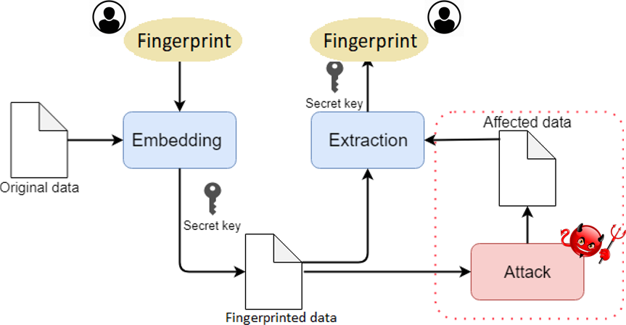
\includegraphics[width=0.38\textwidth]{figures/fingerprint-process.png}
    \caption{Fingerprinting process (applicable to watermarking)}
    \label{fig:process}
\end{figure}

There are multiple methods proposed for watermarking and fingerprinting data and ML models, generally adhering to a 2-step process shown in \Cref{fig:process}: (i) watermark/fingerprint embedding (or insertion) and (ii) watermark/fingerprint detection (or extraction). 
The requirements for such process are:
\begin{enumerate}
    \item recognisable by the owner
    \item not detectable (and removable) by the recipients
    \item robust to the modifications of the object
    \item utility of the object is preserved
\end{enumerate}
To achieve these 4 requirements simultaneously, the techniques need to ensure that the enough marks are embedded to achieve good robustness, but within certain limits to preserve the utility, hence achieving a trade-off between robustness and utility is one of the major challenges in this topic. 

\subsection{Related work}
% data
The first watermarking and fingerprinting techniques for data were developed for multimedia content~\cite{trappe2003anti} and later extended to other domains such as graphs~\cite{piec2014watermarking}, sequential data~\cite{ayday2019robust} and relational datasets~\cite{agrawal2002watermarking,li2005fingerprinting}. 
Our focus is mostly on the later. 
Relational data offers additional challenges compared to multimedia data for watermark/fingerprint embedding such as a limited redundancy of data representation for information (mark) hiding and non-uniformity of data content, i.e. a mix of data attribute types (numerical, text, categorical, etc.). 
% models
Watermarking methods for ML models is a research topic that gained interest in the last 4 years and most of the techniques are designed specifically for Deep Neural Networks for image classification tasks. 
The methods are classified in two main groups depending on the scenario of watermark extraction. 
The \textit{white-box} techniques allow extracting the marks from the model if it is available (shared without and authorisation) in its full form (model parameters, hyperparameters, etc.)~\cite{darvish2019deepsigns,chen2019deepmarks}. 
The \textit{black-box} techniques allow extracting the watermark from the predictions of the model~\cite{chen2019blackmarks,adi2018turning,zhang2018protecting}. 


\section{Preliminary research results}
\subsection{Fingerprinting relational data}
In out work, we address a few shortcomings in the area of fingerprinting relational data.
Firstly, most of the techniques are developed for numerical data in the relational data sets. 
We close this gap by proposing a technique applicable to categorical data, that preserves the original correlations in the data~\cite{sarcevic2020correlation}. 
Secondly, due to the general lack of open-source implementation of fingerprinting techniques for relational data and the lack of conceptual methods for fingerprinting different data types, e.g., categorical, decimal, etc., we have adapted some of the existing techniques to provide the implementation of fingerprinting methodology that can be applied on a variety of data types within relational databases in the form of open-source fingerprinting toolbox\footnote{\url{https://github.com/tanjascats/fingerprinting-toolbox}, version 0.1.0}.  
The toolbox in addition contains implementations of existing fingerprinting methods and framework for simulation of the most common attacks against fingerprinting methods to enable robustness evaluation. 
Using this framework, we evaluated robustness of various techniques from the literature against the attack to obtain the understanding how the choice of the fingerprint parameters affects the resilience of the fingerprint and identify robust scenarios.
\begin{figure}
    \centering
    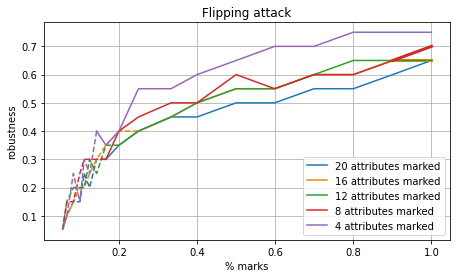
\includegraphics[width=0.38\textwidth]{figures/flipping-german.png}
    \caption[]{Flipping attack on German Credit data\footnotemark}
    \label{fig:robustness}
\end{figure}
\footnotetext{\url{https://archive.ics.uci.edu/ml/datasets/statlog+(german+credit+data)}}
\Cref{fig:robustness} shows such robustness results for our implemented fingerprinting scheme against an exemplary malicious attack, \textit{flipping} the set of random values in the data set.
In an addition to the robustness evaluation, the utility of the fingerprinted data was evaluated to address the trade-off between robustness and preserved data utility that needs to be found for successful fingerprint embedding.~\cite{sarcevic2019evaluation}
The details on our contributions in the fingerprinting relational data and future challenges are summarised in \cite{sarcevic2021fingerprinting}.

\subsection{Watermarking machine learning models}
The work is focusing on a several objectives in the area of watermarking ML models. 
One is the development and application of existing methods in order to assess their differences and shortcomings from the robustness point of view and utility of the fingerprinted or watermarked models. Another objective is focusing on specific attack towards and exploring new vulnerabilities of watermarking schemes. 
Furthermore, in the current research we focus on watermarking methods for special settings such as federated learning, where the existing methods cannot be directly applied. 

\bibliography{bibliography}
\bibliographystyle{IEEEtran}

\end{document}
